\documentclass{article}
\usepackage{graphicx}
\usepackage{fullpage}

\begin{document}
\title{TableSat: Raspberry Pi Edition Documentation \\ \hfill \\ \large Winter 2013: Independent Study Project}
\author{Yiying Li}
\date{\today}

\pagenumbering{roman}
\begin{figure}
\centering
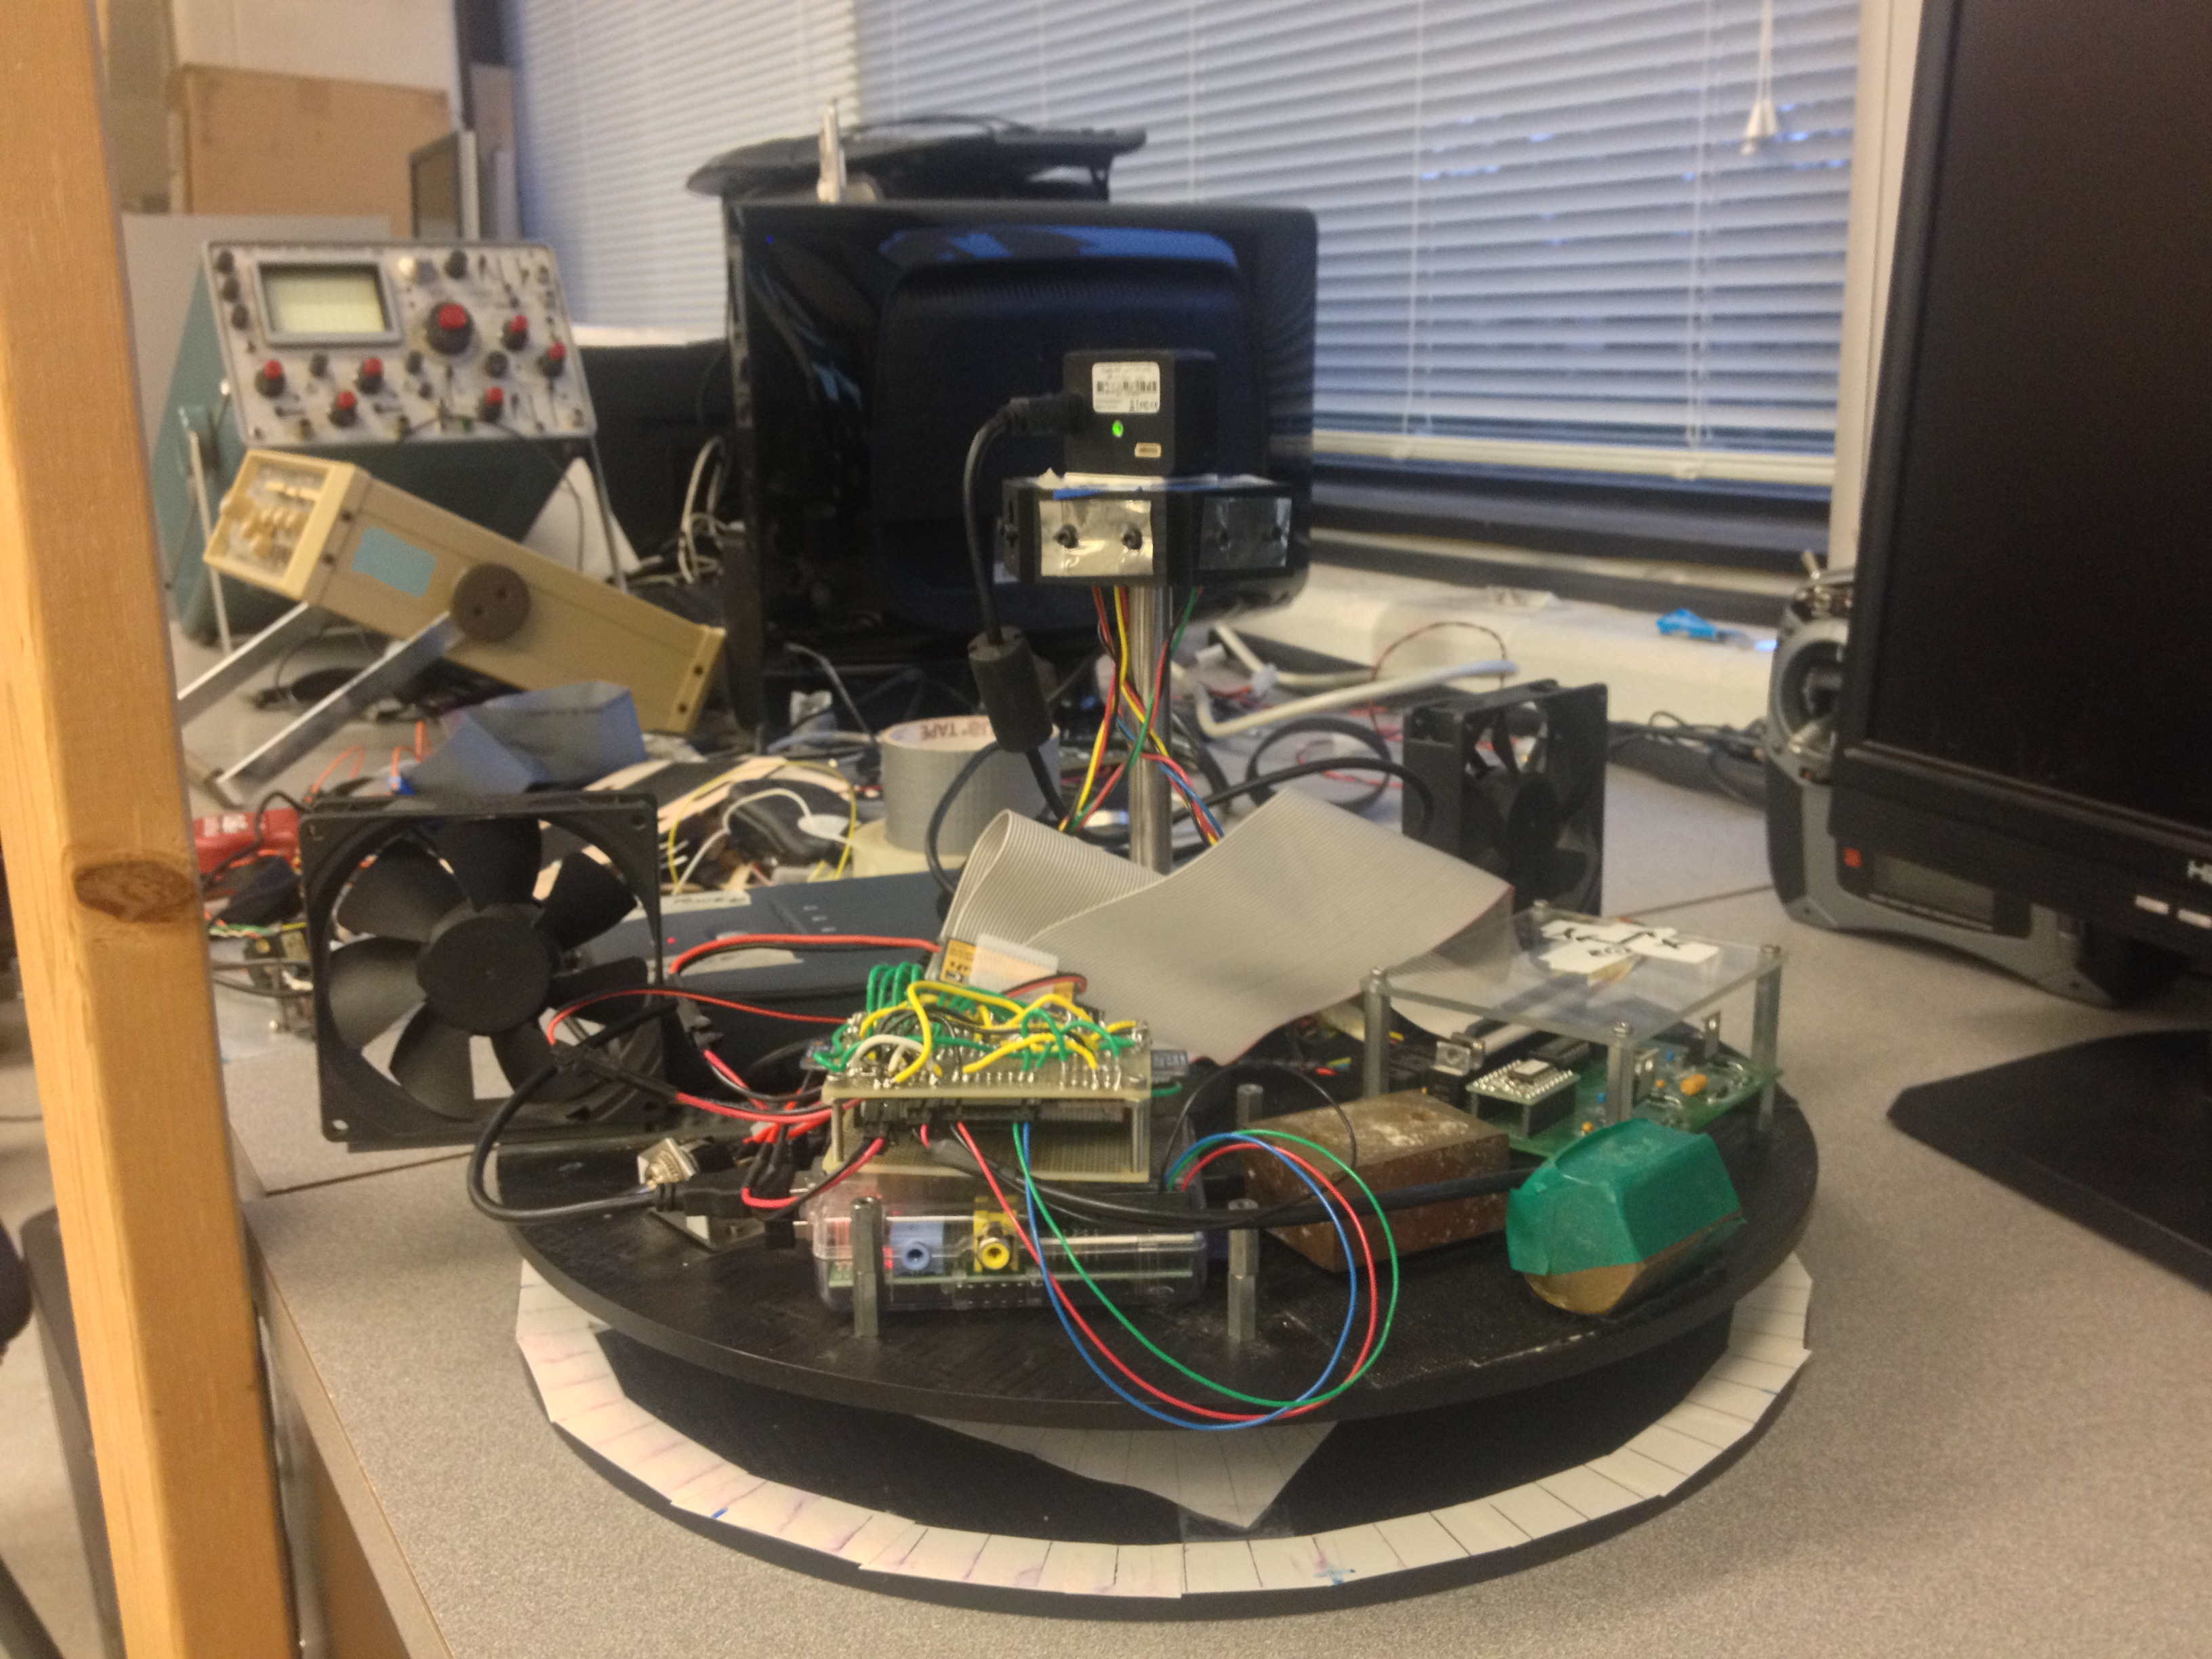
\includegraphics[width=5in]{titlepage.JPG} 
\end{figure}
\maketitle
\thispagestyle{empty}
\pagebreak

\setcounter{page}{1}
\tableofcontents

\pagebreak
\pagenumbering{arabic}

\section{Introduction}
TableSat has been used in Engr151 in many years, however it is quite an older system, and this documentation will deal with how to set up the newer TableSat.
\section{Hardware}
The Raspberry Pi Rev. 2 is the computer for the new TableSat. Rev. 2 is important because the pins of Rev. 1 and Rev. 2 are not the same.
\subsection{Overall Design}
We kept the old interface board and add a newer interface board to allow the Raspberry Pi to communicate with the older interface board without any changes to it.
\subsection{Analog-Digital Converters}
We use ADS1115 16-Bit ADC, 4 Channel with Programmable Gain Amplifier as the analog to digital converters. They can be found at http://www.adafruit.com/products/1085. They have programmable gain however we don't use it on the TableSat as most of our signals are within the 0-5V range. They must be powered by 5V to read the 0-5V range. The main things to note:

\begin{itemize}
    \item There are two ADCs on the same I$^2$C bus
    \begin{itemize}
        \item Both ADC are on the I$^2$C-1 bus, which can be accessed at ``{\tt /dev/i2c-1}'' when the proper drivers have been installed.
        \item Inputs 0-3 are on the first ADC and can be accessed by the slave address 0x48.
        \item Inputs 4-8 are on the second ADC and can be accessed by the slave address 0x49.
    \end{itemize}
    \item The addresses to read and access the ADC are detail in the code file ``{\tt tsat\textunderscore drivers.cpp}''.
    \item The addressing is actually quite complicated therefore it is not detailed in this documentation, all the required address can be found at the top of the code file ``{\tt tsat\textunderscore drivers.cpp}''.
\end{itemize}

\subsection{Digital-Analog Converters}
We use MCP4725 Breakout Board, 12-Bit DAC as the digital to analog converter. They can be found at http://www.adafruit.com/products/935. Each DAC only has one output therefore two are needed. They must be powered at 5V or else they will not output the required 0-5V. The DAC requires a op-amp circuit to to boost the output to the range 0-10V since that is what the old interface board requires. The op-amp that we used isn't a rail-to-rail op-amp, and therefore require around 1V to activate its minimum output, any lower and the op-amp outputs the maximum voltage. Fortunately the DAC contain a EEPROM that we can write a default value to for what the DAC outputs when it hasn't received any commands yet.

\begin{itemize}
    \item There are two DACs on the same I$^2$C bus
    \begin{itemize}
        \item Both DAC are on the I$^2$C-1 bus, which can be accessed at ``{\tt /dev/i2c-1}'' when the proper drivers have been installed.
        \item Inputs 0-3 are on the first DAC and can be accessed by the slave address 0x62.
        \item Inputs 4-8 are on the second DAC and can be accessed by the slave address 0x63.
    \end{itemize}
    \item The address to write the value to is 0x40 for regular access.
    \item The address to write the value to is 0x60 for writing to the EEPROM.
    \begin{itemize}
        \item Students should never be given the option to write to the EEPROM, only in the case of a problem when during boot up the TableSat's fans start spinning should you change the value that is stored in the EEPROM.
    \end{itemize}
\end{itemize}
\subsection{5V regulator}
The 5V regulators we used is just a 5V BEC used in hobby airplanes, this is easily replaced by anything that can take in 19V and output 5V with at least 2A of current. The new interface board has a connector for both 19V out and 5V in, so connecting a different 5V regulator is extremely simple.

\begin{itemize}
    \item The DAC's output will change depending on the 5V, if the regulator is changed, the DAC might output a couple of millivolts more or less than before. This means that the 1V require for the op-amp might change values. More information on how to change this for the software can be found under the Software $\rightarrow$ I$^2$C section
\end{itemize}
\subsection{Circuit Design}
Above is a figure of the circuits and how they all form together. A PCB can be created from this, however its design is not provided with this new version.

\section{Software}
\subsection{Setting up the Raspberry Pi}
\subsubsection{SD Card}
First create the SD card for the Raspberry Pi.

\begin{enumerate}
    \item Plug in the SD card
    \item Check which device is its aka ``{\tt /dev/sdX}'' where X is a letter a-Z.
    \item Run ``{\tt Sudo umount /dev/sdX\#}'' where \# is the partition number, run this for all partition numbers
    \item Run ``{\tt Sudo dd=4M if=imagefile of=/dev/sdX}'', this will take quite a bit of time. At the time of writing this report the image file that was used is named ``{\tt 2013-02-09-wheezy-raspbian.img}''.
    \item Run ``{\tt Sudo sync}'' to force the write to the SD card.
\end{enumerate}

\subsubsection{Raspberry Pi Inital Boot}
Now we have the SD card, plug the it into the Raspberry Pi, as well as a monitor and keyboard.

\begin{enumerate}
    \item You will be greeted with a Raspi-config dialog.
    \item Use the arrow keys to move the ``{\tt expand\textunderscore rootfs}'' option, press enter.
    \item It will tell you that the file system will be enlarged on the next reboot, press enter.
    \item Move to the ``{\tt change\textunderscore pass}'' option, press enter.
    \item It will prompt twice of a new password, press enter when it says ``{\tt Password changed successfully}''.
    \item Move to the ``{\tt change\textunderscore locale}'' option, press enter.
    \item Use the arrow keys to move down to the the option ``{\tt en\textunderscore US.UTF-8 UTF-8}''. Press spacebar you should see an asterisk appear. Press enter.
    \item Select ``{\tt en\textunderscore US.UTF-8}'' on this screen, press enter. It will generate the new locales.
    \item Move to the ``{\tt configure\textunderscore keyboard}'' option, press enter.
    \item It should already highlight ``{\tt Generic 105-key (Intl) PC}'', just press enter.
    \item Select Other, press enter, select ``{\tt English (US)}'', press enter.
    \item Select ``{\tt English (US)}'' again, press enter. Keep pressing enter until you arrive at the Raspi-config main page again.
    \item Select ``{\tt boot\textunderscore behaviour}'', press enter, choose ``{\tt No}'', press enter.
    \item Select ``{\tt Finish}'', press enter, choose ``{\tt Yes}'' for reboot, press enter.
 \end{enumerate}

The username is ``{\tt pi}'', and the password is what you just set above.

\subsubsection{Setting up I$^2$C Drivers}
Now we need to install the I$^2$C drivers.

\begin{enumerate}
    \item Connect the Raspberry Pi to the internet using an ethernet connection
    \item Run ``{\tt sudo apt-get update}''
    \item Run ``{\tt sudo apt-get upgrade}''
    \item Run ``{\tt sudo apt-get install i2c-dev}''
    \item Edit the file ``{\tt /etc/modules}'' (need to use ``{\tt sudo}'') add two lines ``{\tt i2c-dev}'' and ``{\tt i2c-bcm2708}'' The file should look like the following after you add those lines:

    { \tt
    snd-bcm2835 \\
    i2c-dev \\
    i2c-bcm2708 \\
    }
    \item Run ``{\tt sudo usermod -aG i2c pi}'', this will add the user pi to the i2c group so you can access the i2c devices without using ``{\tt sudo}''.
\end{enumerate}

\subsubsection{Setting up WiFi}
We not need to set up the WiFi. Power down the Raspberry Pi, as plugging in the USB WiFi adapter will reboot the Pi anyways.

\begin{enumerate}
    \item Edit the file ``{\tt /etc/network/interfaces}'' (need to use ``{\tt sudo}''). Change the file to look like:

    {\tt
    auto lo \\
    \hfill \\
    iface lo inet loopback \\
    iface eth0 inet dhcp \\
    \hfill \\
    allow-hotplug wlan0 \\
    auto wlan0 \\
    iface wlan0 inet manual \\
    wpa-roam /etc/wpa\textunderscore supplicant/wpa\textunderscore supplicant.conf \\
    iface default inet dhcp
    }

    \item Edit the file ``{\tt /etc/wpa\textunderscore supplicant/wpa\textunderscore supplicant}'' to look like replacing ESSID with the ESSID of the network:

    {\tt
    ctrl\textunderscore interface=DIR=/var/run/wpa\textunderscore supplicant GROUP=netdev \\
    \hfill \\
    network=\{ \\
    ssid="ESSID" \\
    key\textunderscore mgmt=NONE \\
    priority=-999 \\
    \} \\
    }
\end{enumerate}

Reboot and the Pi should now connect to the WiFi network. If it doesn't double check the ``{\tt wpa\textunderscore supplicant.conf}'' to make sure it is correct. If connecting to a WEP or WPA2 network look at examples online, they are easy to find.

\subsubsection{Camera Setup}
We have to install the drivers for the cameras as well as make sure standard users can access the camera without using ``{\tt sudo}''.

\begin{enumerate}
    \item Run ``{\tt sudo apt-get install libdc1394-22-dev}''.
    \item Run ``{\tt cd /opt/vc/src/hello\textunderscore pi/libs/ilclient}''.
    \item Run ``{\tt make}''.
    \item Copy the file ``{\tt 40-pgr.rules}'' to the Pi using SCP.
    \item Copy the file ``{\tt 40-pgr.rules}'' to the directory ``{\tt /etc/udev/rules.d/}''
    \item Copy the tar ``{\tt udt.sdk.4.11.tar.gz}'' to the Pi using SCP.
    \item Extract the tar using ``{\tt tar xvaf udt.sdk.4.11.tar.gz}''.
    \item cd into the directory using ``{\tt cd udt4}''.
    \item Run ``{\tt make -e arch=arm}''.
    \item cd into ``{\tt src}''
    \item Run ``{\tt sudo mkdir /usr/include/udt}''
    \item Run ``{\tt sudo cp *.h /usr/include/udt/.}''
    \item Run ``{\tt sudo cp libudt.* /usr/lib/.}''
\end{enumerate}
Now the camera should be registered as the video group when it gets connected, and since we add new users to the video group they can access the camera without using ``{\tt sudo}''.
\\
\\
\emph{NOTE: The camera server will not work until you finish the server step detailed in Software $\rightarrow$ Setting up the ``{\tt Server}'' $\rightarrow$ Vision.}

\subsubsection{User Creating Scripts}
I provide two scripts to create and delete users ``{\tt createUsers.py}'' and ``{\tt deleteUsers.py}''. They are both python scripts.
\begin{itemize}
    \item They are both used the same way ``{\tt ./createUsers.py file}'', where file is the file containing the usernames, each username seperated by a newline.
    \item ``{\tt ./createUsers.py}'':

    \begin{itemize}
        \item Inside this python script there is a field for the default password, change this to use a different default password.
        \item This script will automatically add users to the i2c and video groups so they can interface with the I$^2$C buses and the camera, however they are not system admins and cannot to anything with ``{\tt sudo}''.
    \end{itemize}

    \item ``{\tt ./deleteUsers.py}'':

    \begin{itemize}
        \item This script deletes all the users from the Pi, it also removes all their files and home directories. Don't use this unless you are sure you want to delete everyone's files.
    \end{itemize}
\end{itemize}

\subsection{Setting up the ``{\tt Server}''}
\subsubsection{Cross Compiling}
This is to set up a cross compiler to the Pi

\begin{enumerate}
    \item Run ``{\tt sudo apt-get install bison flex gperf texinfo gawk libtool automake libncurses5-dev subversion
    }''.
    \item cd into the directory using ``{\tt cd crosstool-ng-1.18.0}''.
    \item Run ``{\tt ./configure --prefix=/opt/cross}''.
    \item Run ``{\tt make}'' then ``{\tt sudo make install}''.
    \item cd into back into original directory
    \item Make a dir for staging ``{\tt mkdir cross\textunderscore stage}''.
    \item Run ``{\tt /opt/cross/bin/ct-ng menuconfig}''
    \item Go to ``Paths and misc'', enable ``Try features marked as EXPERIMENTAL'' (spacebar).
    \item Change the prefix director to ``{\tt /opt/cross/x-tools/\$\{CT\textunderscore TARGET\}}''
    \item Go back to the main menu (Esc) and select ``Target options''.
    \item Change the ``Target architecture'' to ``arm''.
    \item Go back to the main menu and select ``Operating system''.
    \item Change ``Target OS'' to ``linux''.
    \item Go back to the main menu and select ``Binary utilities''.
    \item Change ``binutils version'' to the first one that isn't marked as experimental.
    \item Go back to the main menu and select ``C compiler''.
    \item Change ``gcc version'' to the top one.
    \item Exit and save changes.
    \item Run ``{\tt sudo chmod a+rw /opt/cross}''
    \item Run ``{\tt /opt/cross/bin/ct-ng build}'', this will take a while.
    \item Run ``{\tt sudo ln -s /opt/cross/x-tools/arm-unknown-linux-gnueabi/bin/ \\ arm-unknown-linux-gnueabi-g++ /usr/bin/rpi-g++}''
    \item cd into back into original directory
    \item cp the file ``{\tt i2c-dev.h}'' to the cross compile root by running: \\
    ``{\tt cp i2c-dev.h /opt/cross/x-tools/arm-unknown-linux-gnueabi/arm-unknown-linux-gnueabi/ \\ sysroot/usr/include/linux/.}''
\end{enumerate}

\subsubsection{Vision}
We need to set up the server for the computer vision.

\begin{enumerate}
    \item Run ``{\tt sudo apt-get install pkg-configsudo}''.
    \item Extract the tar using ``{\tt tar xvaf udt.sdk.4.11.tar.gz}''
    \item cd into the directory using ``{\tt cd udt4}''.
    \item Run ``{\tt make}''.
    \item cd into ``{\tt src}''
    \item Run ``{\tt sudo mkdir /usr/include/udt}''
    \item Run ``{\tt sudo cp *.h /usr/include/udt/.}''
    \item Run ``{\tt sudo cp libudt.* /usr/lib/.}''
    \item cd into back into original directory
    \item Download the ffmepg files from http://www.ffmpeg.org/releases/ffmpeg-snapshot.tar.bz2.
    \item Extract the tar using ``{\tt tar xvaf ffmpeg-snapshot.tar.bz2}''.
    \item cd into the directory using ``{\tt cd ffmpeg}''.
    \item Run ``{\tt sudo apt-get install yasm}''.
    \item Run ``{\tt ./configure}''.
    \item Run ``{\tt make}''.
    \item Run ``{\tt sudo make install}''.
    \item Run ``{\tt sudo apt-get install cmake}''.
    \item Run ``{\tt sudo apt-get install libgtk2.0-dev}''.
    \item cd into back into original directory
    \item Download the latest OpenCV, untar it cd into that directory. Skip the rest if OpenCV is already installed.
    \item Run ``{\tt mkdir BUILD}''.
    \item Run ``{\tt cd BUILD}''.
    \item Run ``{\tt cmake ..}''.
    \item Run ``{\tt make}''.
    \item Run ``{\tt sudo make install}''.
\end{enumerate}

\subsection{The Code}
All of the code are located in the ``{\tt src}'' folder.
\subsubsection{I$^2$C Userspace Libraries}
The I$^2$C drivers for the TableSat are located in the files ``{\tt tsat\textunderscore drivers.cpp}'' and ``{\tt tsat\textunderscore drivers.h}'' in the source directory.
\begin{itemize}
    \item The ``{\tt Makefile}'' will automatically make the file ``{\tt tsat\textunderscore drivers.a}''. If you want to make this file on the Pi without cross compiling then you need to run 
    \begin{enumerate}
        \item ``{\tt g++ -Wall tsat\textunderscore drivers.cpp -c -o tsat\textunderscore driver.o}''
        \item ``{\tt ar crv tsat\textunderscore drivers.a tsat\textunderscore drivers.o}''
    \end{enumerate}
    \item You should only make the file ``{\tt tsat\textunderscore drivers.a}'' and ``{\tt tsat\textunderscore drivers.h}'' available to the students as I'm afraid that they will try to write to the EEPROM if they can see the source code. If they are only given the ``{\tt .a}'' file they can't see the source.
    \item The command they would use to compile would then be:

    ``{\tt g++ main.cpp tsat\textunderscore drivers.a -o program}''
    \item The source file ``{\tt tsat\textunderscore drivers.cpp}'' contains a tunable parameter that is the number require to output 1V to the fans to make then stop due to the problem with the op-amp. This number has been shown to work with the current 5V regulator, however might have to be changed if a new 5V regulator is used.

    \begin{itemize}
        \item ``{\tt command\textunderscore fan.cpp/.h}'': contains the command\textunderscore fan example.
        \item ``{\tt read\textunderscore gyro.cpp/.h}'': contains the read\textunderscore gyro example.
        \item The makefile will also make ``{\tt command\textunderscore fan\textunderscore eeprom}'': this program is used to write to the EEPROM. Students shouldn't have this program in case they set the EEPROM to max and when the TableSat boots it will start with max fan.
    \end{itemize}
\end{itemize}
\subsubsection{Computer Vision}
The computer vision are split up into Server and Client code. The server being the code that runs on the Pi and the client being the code that runs on another computer.
\subsubsection{Server}
You should not distribute the source code of the ``{\tt camserver}'' to the students that want to use it. Only the executable should be released. This is due to the face that the GPU is extremely volatile and if someone changes the GPU code it could mess up the GPU until a reboot can be done.

The ``{\tt Makefile}'' will create this program only using the command ``{\tt make camserver}''. \emph{THIS HAS TO BE DONE ON THE PI}, this is because there are GPU code that is extremely hard to pull into the cross compiling environment.

How to run ``{\tt camserver}'':  ``{\tt ./camserver bitrate}'' where the bitrate is the average bitrate you want for the video stream, 20000000 is extremely high quality video and this is the max, defaults to the lowest possible bitrate. ``{\tt ./camserver bitrate > /dev/null}'' will pipe the output to nothing, this is useful as the ssh connection takes bandwidth as well.

\begin{itemize}
    \item ``{\tt camserver.cpp/.h}'': contains the GPU encoding code.
    \item ``{\tt udtComm.cpp/.h}'':
    \begin{itemize}
        \item This code contains the code required to set up the udt server, its not really meant as a library more of helper functions.
        \item Again this code (both .cpp and .h) shouldn't be distributed, however it can be as there isn't too much harm to any physical systems, it might be nice to keep the complicated nature of it away from students.
    \end{itemize}
    \item ``{\tt camera.cpp/.h} + {\tt cameraconstants.h}'': contains the code to grab images from the camera.
\end{itemize}

\subsubsection{Client}
\begin{itemize}
    \item ``{\tt RPiDecode.cpp/.h}'':
    \begin{itemize}
        \item This is the code that contains all the code for receiving and and decoding the images
        \item Again this code (.cpp only) shouldn't be distributed, however it can be as there isn't too much harm to any physical systems, it might be nice to keep the complicated nature of it away from students.
    \end{itemize}
    \item ``{\tt udtComm.cpp/.h}'':
    \begin{itemize}
        \item This code contains the code required to set up the udt server, its not really meant as a library more of helper functions.
        \item Again this code (both .cpp and .h) shouldn't be distributed, however it can be as there isn't too much harm to any physical systems, it might be nice to keep the complicated nature of it away from students.
    \end{itemize}
    \item ``{\tt RPiDecode.a}'' + ``{\tt RPiDecode.h}'':
    \begin{itemize}
        \item These are the files that should be given to the students who want to work on vision. 
        \item The example program to display images is located in ``{\tt camclient.cpp}''. To compile use: ``{\tt g++ -D\textunderscore \textunderscore STDC\textunderscore CONSTANT\textunderscore MACROS -Wall camclient.cpp RPiDecode.a -o camclient `pkg-config \\ libavcodec libavutil libswscale opencv --cflags --libs` -ludt}''
        \item Everything in the compile line is strictly required.
        \item ``{\tt -D\textunderscore \textunderscore STDC\textunderscore CONSTANT\textunderscore MACROS}'' is required as there is a bug that says a certain constant isn't defined in the FFMPEG libraries.
        \item ``{\tt pkg-config *}'' and ``{\tt -ludt}'' are required for linking.
    \end{itemize}
\end{itemize}

\end{document}